\input{/home/diego/Documents/Licenciatura/LatexBasic/Preamble_general}

%%%%%%%%%%%%%%%%%%%%%%%%%%%%%%%%%%%%%%%%%%%%%%%%%%%%%%%%%%%
\usepackage{fancyhdr}%formato de pagina
\pagestyle{fancy}%colocar la pagina con el formato deseado
\fancyhead{}
\fancyhead[L]{\footnotesize{Electrónica Digital}}
\fancyhead[C]{Simulacion 2}
\fancyhead[R]{\footnotesize{\thepage}}
%\fancyhead[LO,RE]{Cálculo 3}
%\fancyhead[RO,LE]{\footnotesize{\thepage}}
\fancyfoot{}
\fancyfoot[L]{Diego Sarceño}
%\fancyfoot[LO,RE]{Diego Sarceño}
%%%%%%%%%%%%%%%%%%%%%%%%%%%%%%%%%%%%%%%%%%%%%%%%%%%%%%%%%%%

\begin{document}
\begin{titlepage}
% AUTOR: Diego Sarceño

% ENCABEZADO DE TRABAJOS CON LOGO DE LA UNIDAD ACADÉMICA

% ENCABEZADO LOGO COLOR
%\begin{tabulary}{20cm}{Lp{0.9cm}p{6.1cm}}
%Universidad de San Carlos de Guatemala & & \multirow{4}{8cm}{\hfill %\includegraphics[scale=0.5]{ECFM.png}}\\            % Logo de la unidad academica
%Escuela de Ciencias Físicas y Matemáticas & \hfill & \\
%Diego Sarceño 201900109 & \hfill & \\
%Análisis de Variable Compleja 1 & \hfill & \\
%\today & & \\
%\end{tabulary}\\[0.25cm]


% ENCABEZADO LOGOS
\begin{tabulary}{20cm}{LLCRR}
\multirow{4}{2.3cm}{\includegraphics[scale=0.13]{/home/diego/Documents/Licenciatura/LatexBasic/ECFM.pdf}} & Universidad de San Carlos de Guatemala  & & & \multirow{4}{5cm}{\hfill \includegraphics[scale=0.082]{/home/diego/Documents/Licenciatura/LatexBasic/USAC.pdf}}\tabularnewline
 & Escuela de Ciencias Físicas y Matemáticas & \hfill &  & \tabularnewline
 & Mecánica 3 & \hfill ~~ &   & \tabularnewline
 & Diego Sarceño 201900109 & &  & \tabularnewline
 & \today &  & & \tabularnewline
\end{tabulary}\\[0.75cm]

{\hrule height 1.5pt} \vspace{0.1cm}
\begin{tabulary}{21cm}{p{6cm}p{7cm}p{8cm}}
    \hfill & \huge{\scshape{Tarea 4}} & \hfill
\end{tabulary}
{\hrule height 1.5pt} 
\vspace{0.5cm}


\noindent
El archivo de \LaTeX esta disponible en el repositorio de \href{https://github.com/DSarceno/Semestre6/tree/main/Electr\%C3\%B3nica\%20Digital/Tarea\%202}{GitHub}.


 % Tarea 1 ED
 

\section{Bitácoras}

\subsection{Bitácora 1}

Se inició creando el primer sumador completo, con sus respectivas compuertas XOR, OR y AND. El primer set de switches representa la primera entrada de $4$ bits, mientras que el segundo representa la otra entrada de $4$ bits. El primer bit de acarreo esta representado por medio de tierra ($0V$).


\begin{figure}[H]
	\centering
	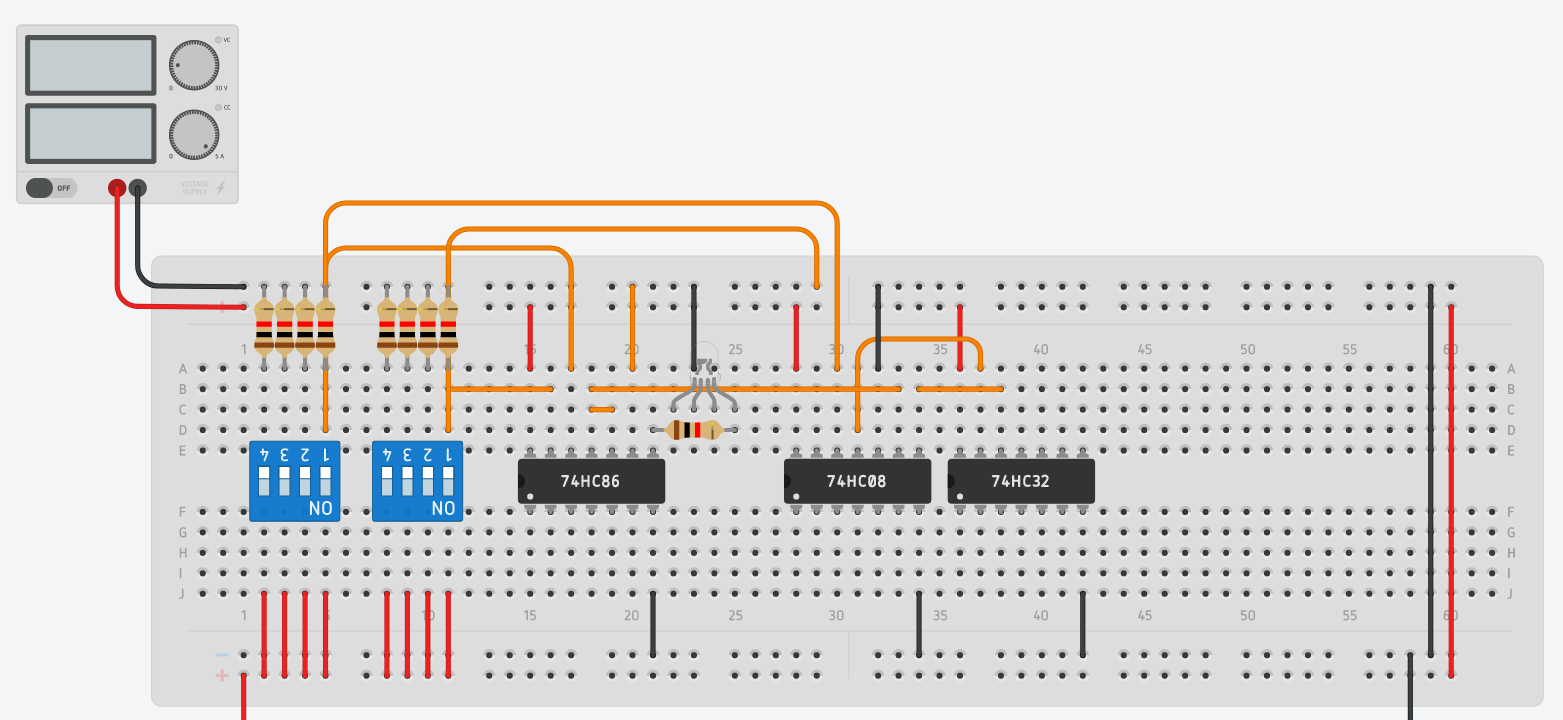
\includegraphics[scale=0.25]{Images/Parte1SC1.png}
	\caption{Primera suma con su correspondiente bit de acarreo.}
	\label{p1sc1}
\end{figure}

\subsection{Bitácora 2}

Se realizaron los sumadores de los dos bits restantes y sus correspondientes bits de acarreo. Se tiene un problema con los bits de acarreo y el de desbordamiento, puesto que no encienden todos.

\begin{figure}[H]
	\centering
	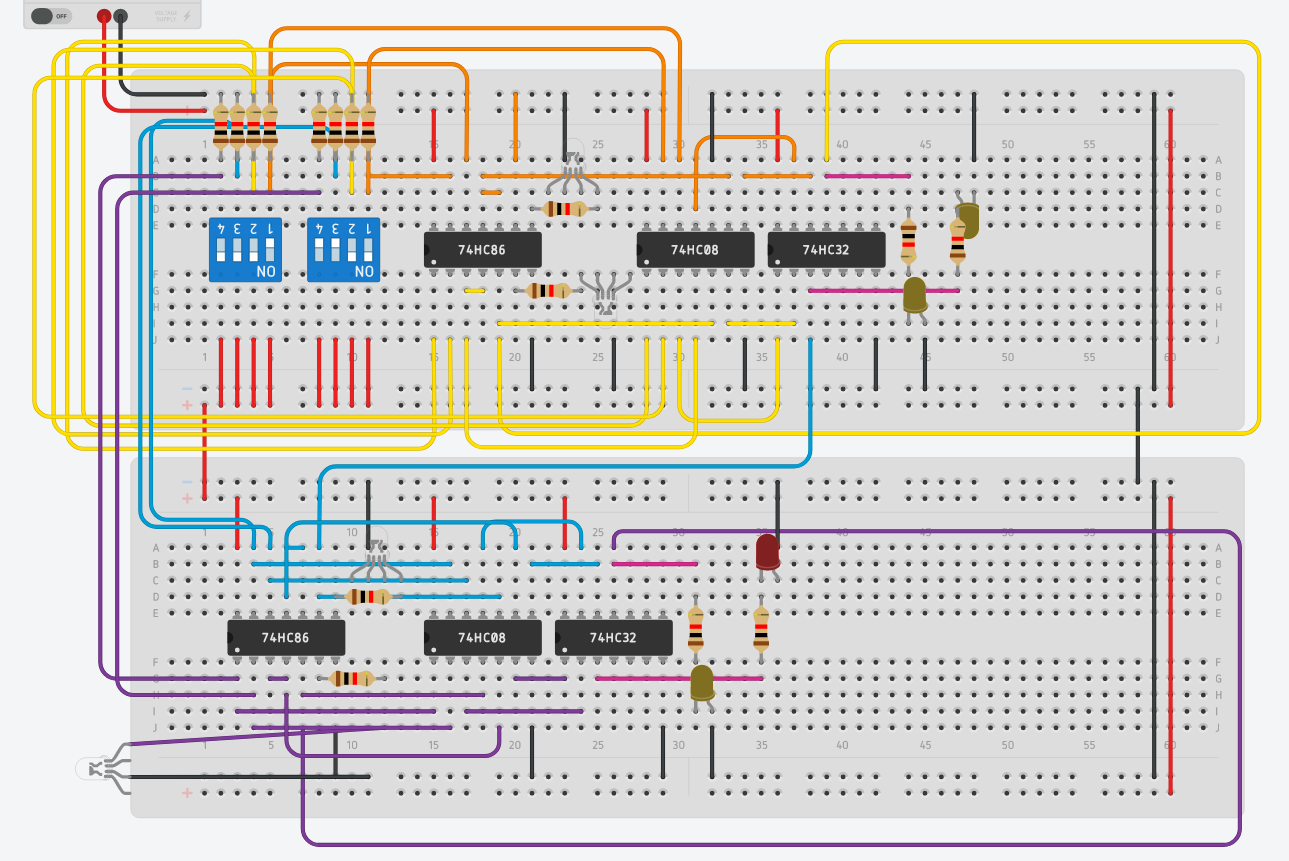
\includegraphics[scale=0.25]{Images/Parte1SC2.png}
	\caption{Circuito Sumador completo para dos sets de $4$ bits con sus bits de acarreo y desbordamiento.}
	\label{p1sc2}
\end{figure}


























\end{titlepage}
\end{document}
